
\subsection{Benutzung des Clients}
\label{sec:benutz-des-clients}
Nach Konfiguration des Clients muss zunächst der Server gestartet
werden, da der Client eine funktionierende Verbindung zum Server
voraussetzt. Ist keine vorhanden, bricht er die Programmausführung ab.
Nach Start des Servers  positioniert man den Roboter in der Mitte des
Raumes, in dem die Ballsuche stattfinden soll. Anschließend schaltet
man den Roboter ein und startet den Client mit der
Stapelverarbeitungsdatei \verb|Start.bat|. Der Client startet nun und
nimm zunächst soviele Rotationen um die eigene Ache vor, wie in der
\verb|config.cfg| festgelegt worden sind. Diese dienen dazu, den
Sonar-Partikelfilter zu initialisieren, sodass der Client dann die
Position des Roboters im Raum bestimmen kann. Nach erfolgreicher
Initialisierung verbindet sich der Client mit den Server und wartet,
bis dieser die Suche startet. Sobald vom Server die Suche gestartet
wurde, wird der Client vom Server eine Liste von Punkten anfordern,
die er dann abfahren wird. Gleichzeitig öffnet sich ein Fenster, dass
das aktuelle Bild der Kamera zeigt. Es wird während der gesamten Suche
ständig aktualisiert. \\\\
Ab diesen Zeitpunkt muss man als Benutzer
nur noch den Ablauf überwachen, falls es unerwarteterweise zu
Kollisionen mit der Wand oder anderen Robotern kommt. Dies sollte zwar
aufgrund der vom Server vorgenommen Kollisionerkennung nicht
passieren, allerdings lassen sich ,,false Positives'' nicht generell
ausschließen, mehr dazu im nächsten Kapitel. Erkennt der Client
schließlich einen Ball im aktuellen Kamerabild, wird der Ball im Bild
markiert:
\begin{nofloat}{figure}\centering
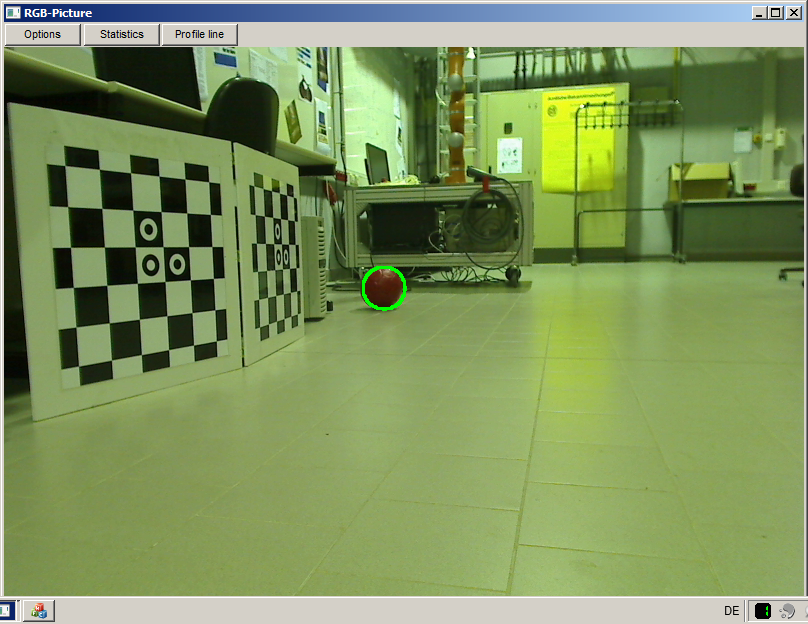
\includegraphics[width=0.75\linewidth]{bilder/balldetect}
\caption{Kamerabild bei erfolgreicher Ballerkennung}  
\end{nofloat}

Anschließend wird aus der mit den Sonar-Partikelfilter ermittelten
Position des Roboters im Raum und von der Ballerkennung zurückgebenen
Entfernung und Winkel vom Ball zum Roboter die Position des Balls im
Raum bestimmt und an den Server übermittelt. Dieser weiß nun, dass die
Ballsuche erfolgreich beendet ist und schickt allen verbundenen
Clients eine Aufforderung die Suche zu beenden. In der Folge stoppen
die Clients die Suche.

%%% Local Variables: 
%%% mode: latex
%%% TeX-master: "template"
%%% End: 
